%%%%%%%%%%%%%%%%%%%%%%%%%%%%%%%%%%%%%%%%%%%%%%%%%%%%%%%%%%%%%%%%%%%%%%%%%%%
%
% Plantilla para un artículo en LaTeX en espa\~nol.
%
%%%%%%%%%%%%%%%%%%%%%%%%%%%%%%%%%%%%%%%%%%%%%%%%%%%%%%%%%%%%%%%%%%%%%%%%%%%

\documentclass{article}


% Esto es para poder escribir acentos directamente:
\usepackage[T1]{fontenc}

\usepackage[utf8]{inputenc}

% Esto es para que el LaTeX sepa que el texto está en espa\~nol:
\usepackage[spanish]{babel}
% Esto es para que se pueda crear el índice
%\usepackage{makeidx}
% Paquetes de la AMS:
\usepackage{amsmath, amsthm, amsfonts}
% para poder poner una hoja apaisada
\usepackage{lscape}
%para incluir graficos
\usepackage{graphicx}
%para permitir que la imagen este donde yo quiero y no en otro lugar
\usepackage{float}
% para hipertexto
%\usepackage{url}
% para poder envolver imágenes con texto
\usepackage{wrapfig}
%para los apéndices
\usepackage[titletoc]{appendix}
% Esto es para poder modificar las dimensiones del texto
\usepackage{geometry}
\geometry{a4paper}

%para usar hipertexto en las referencias
\usepackage{hyperref}
\hypersetup{
    colorlinks,
    citecolor=black,
    filecolor=black,
    linkcolor=black,
    urlcolor=black
}

\usepackage{fancyhdr}

\pagestyle{fancy}
\fancyhf{}
\rhead{Informe de las 100 horas}
\lhead{Practica Profesional Supervisada}
\rfoot{\thepage}
\lfoot{FCEFyN - UNC}


\graphicspath{ {Imagenes/} }

% Teoremas
%--------------------------------------------------------------------------
\newtheorem{thm}{Teorema}[section]
\newtheorem{cor}[thm]{Corolario}
\newtheorem{lem}[thm]{Lema}
\newtheorem{prop}[thm]{Proposición}
\theoremstyle{definition}
\newtheorem{defn}[thm]{Definición}
\theoremstyle{remark}
\newtheorem{rem}[thm]{Observación}

% Atajos.
% Se pueden definir comandos nuevos para acortar cosas que se usan
% frecuentemente. Como ejemplo, aquí se definen la R y la Z dobles que
% suelen representar a los conjuntos de números reales y enteros.
%--------------------------------------------------------------------------

\def\RR{\mathbb{R}}
\def\ZZ{\mathbb{Z}}

% De la misma forma se pueden definir comandos con argumentos. Por
% ejemplo, aquí definimos un comando para escribir el valor absoluto
% de algo más fácilmente.
%--------------------------------------------------------------------------
\newcommand{\abs}[1]{\left\vert#1\right\vert}
\newcommand{\summary}[1]{\addtocontents{toc}{#1\par}}

% Operadores.
% Los operadores nuevos deben definirse como tales para que aparezcan
% correctamente. Como ejemplo definimos en jacobiano:
%--------------------------------------------------------------------------
\DeclareMathOperator{\Jac}{Jac}

%--------------------------------------------------------------------------
\title{\underline{Práctica Profesional Supervisada} \\
\large \underline{Informe de las 100 horas} \\
\huge \textbf{ \\ Plataforma Concentradora de Sensores y Eventos Digitales} \\ }
\author{Autores: Ignacio Sambataro, Luciano Mantovani\\ \\
  \large Tutor: PhD. Ing. Orlando Micolini \\
  \large Supervisor: Ing. Maximiliano Eschoyez
 % \small Facultad de Ciencias Exactas, Físicas y Naturales\\
 % \small Laboratorio de Arquitectura de Computadoras\\
 % \small Universidad Nacional de Cordoba\\
  \date{}
}



%\makeindex
\begin{document}
\thispagestyle{empty}
\maketitle
\thispagestyle{empty}
\begin{figure}[H]
\centering

\includegraphics[width=10cm, height = 3.2cm]{Escudo}
\end{figure}

\begin{center}
\small Facultad de Ciencias Exactas, Físicas y Naturales
\end{center}

\begin{center}
\small Laboratorio de Arquitectura de Computadoras
\end{center}

\begin{center}
\small Año 2015 \\
\end{center}

\pagebreak

\thispagestyle{empty}
%resumen
\abstract{En este informe se describen las primeras 100 horas de trabajo de la Práctica Profesional Supervisada. Se comenzó un proyecto nuevo, sugerido por el director, Orlando Micolini, y se trabajo todo el tiempo en el Laboratorio de Arquitectura de Computadoras. Se documentaron los requerimientos, la etapa de investigación, los dise\~nos de hardware y software hasta el momento, y las implementaciones que se llegaron a lograr. Lo que se llego a implementar se hizo en una placa de desarrollo prestada. Las razones de utilización de esta placa se explican en el documento. Algunos requerimientos básicos llegaron a cumplirse dentro de las 100 horas, pero solamente prototipos de prueba en la placa de desarrollo. El primer prototipo real tiene la mayor parte del dise\~no de hardware y software hecho, pero todavía no esta implementado. }

%salto de página
\thispagestyle{empty}
\clearpage
\thispagestyle{empty}
\tableofcontents
\thispagestyle{empty}
\clearpage

\setcounter{page}{1}
%introducción
\section{Introducción} % (fold)
\label{sec:introduccion}

Esta practica esta orientada al diseño y la construcción de un sistema embebido que concentre las señales de varios sensores y varias fuentes de eventos digitales. La idea es que un sistema embebido de uso especifico pueda tercerizar la tarea de obtener, convertir y procesar una señal de uno o varios sensor o una o varias fuente de eventos digitales.

Surgió de la problematica de algunos proyectos dentro del Laboratorio de Arquitectura de Computadoras que compartían el mismo problema. La necesidad de un sistema que genéricamente obtenga las señales de los sensores y la pueda transmitir al sistema principal, ya convertidas. Además de un contador de eventos que no requiera del uso de interrupciones por software.

En este informe cubrimos los avances hechos en las primeras 100 horas de trabajo en el proyecto.

% section introducción (end)

%requerimientos
\section{Planteo de Requerimientos} % (fold)
\label{sec:planteo_de_requerimientos}

\subsubsection{Requerimientos principales} % (fold)
\label{ssub:requerimientos_principales}

\begin{itemize}
  \item Leer de 4 a 8 señales analógicas y convertirlas a digital.
  \item Contar eventos con 3 o 4 contadores distintos.
  \item Transmitir los datos digitales a través de un protocolo serial a alguna otra placa o procesador.
\end{itemize}

% subsubsection requerimientos_principales (end)

\subsubsection{Requerimientos Secundarios} % (fold)
\label{ssub:requerimientos_secundarios}

\begin{itemize}
  \item Lograr el menor consumo posible.
  \item Buscar la mejor inmunidad al ruido, con una distancia de la placa a los sensores de hasta un máximo de 10 metros.
  \item Lograr un producto lo más pequeño posible.
  \item Lograr un producto programable
\end{itemize}

% subsubsection requerimientos_secundarios (end)

% section requerimientos (end)

%investigación
\section{Investigación} % (fold)
\label{sec:investigacion}

La etapa de investigación consistió en encontrar un microcontrolador que satisfaga la mayor cantidad de requerimientos principales. El sistema entero consiste en interactuar con el núcleo, que es el microcontrolador, por lo que esta etapa requirió de análisis detallado de las opciones con las se contaba. En el cuadro\ref{tab:microcontroladores} se pueden ver los microcontroladores considerados en la etapa de selección.

% Table generated by Excel2LaTeX from sheet 'Sheet1'
\clearpage

\begin{landscape} % TABLA DE MICROS

\begin{table}[!]
\centering
\begin{flushleft}
% Table generated by Excel2LaTeX from sheet 'Sheet1'
\scalebox{0.67}{
\begin{tabular}{|c|c|c|c|c|c|c|c|c|c|c|c|c|}
\hline
Fabricante & Modelo & RAM(K) & canales ADC & Referencia & Resolución & ganancia & Contadores & low power & puerto serie & Dimension (') &   Pins &   Us\$ \\
\hline
 Intel & 8XC51GB &    256 &      8 &    GND & 8 bits &     no & 3 (16 bits) &     si & salida y entrada RS232 &      N &     32 &      N \\
\hline
Silicon Labs & C8051F352 &    768 &      8 & DIF/GND & 24 bits &   128x & 4 (16 bits) &     si & Smbus/$I^{2}$C, UART, SPI & 0,35x0,35 &     32 &    2,3 \\
\hline
 Atmel & AT89C5115 &    256 &      8 &    GND & 8/10 bits &     no & 3 (16 bits) &     si & UART (3 modos Full Duplex) & 0,34x0,34 &     32 &     10 \\
\hline
Microchip & PIC18F4550 &     32 &     13 &    GND & 10 bits &     no & 4(8 y 16 bits) &     si & SPI, $I^{2}$C, UART/USART, USB & 0,47x0,47 &     44 &   5,36 \\
\hline
   Nec & PD78C17 &   1024 &      8 &    GND & 8 bits &     no & 2 (8 bits) &     si & Msbus/$I^{2}$C & 0,92x0,70 &     64 &      N \\
\hline
 Maxim & DS4830 & 1024x16 &     16 & DIF/GND & 13 bits &     no & 2(16 bits) &     si & SPI, $I^{2}$C & 0,2x0,2 &     40 &    7,5 \\
\hline
   NXP & LPC1110 &      4 &      8 &    GND & 10 bits &     no & 2(32 bits) &     si & $I^{2}$C, UART, Soporte RS-485 & 0,42x0,51 &     20 &    2,5 \\
\hline
 Atmel & ATSAM3A8C &    256 &     16 & DIF/GND & 12 bits &     no & 9(32 bits) &     si & USB, SPI & 0,63x0,63 &     63 &    2,4 \\
\hline
 Atmel & ATSAM3S1A &     64 &      8 & DIF/GND & 10/12 bits & 1x,2x,4x & 3(16 bits) &     si & USB, $I^{2}$C, SPI & 0,35x0,35 &     44 &    2,5 \\
\hline
 Atmel & ATSAM3S1C &     16 &     16 & DIF/GND & 10/12 bits & 1x,2x,4x & 6(16 bits) &     si & USB, $I^{2}$C, SPI & 0,63x0,63 &     74 &    2,5 \\
\hline
 Atmel & ATSAMD21J &    256 &     20 & DIF/GND & 12 bits &    16x & 5 (16 bits) &     si & 1 USB 2.0 + 6 $I^{2}$C/USART/SPI & 0,47x0,47 &     64 &      3 \\
\hline
 Atmel & ATSAMD21G &    256 &     14 & DIF/GND & 12 bits &    16x & 3 (16 bits) &     si & 1 USB 2.0 + 6 $I^{2}$C/USART/SPI & 0,35x0,35 &     48 &    2,5 \\
\hline
 Atmel & ATSAMD21E &    256 &     10 & DIF/GND & 12 bits &    16x & 3 (16 bits) &     si & 1 USB 2.0 + 4 $I^{2}$C/USART/SPI & 0,35x0,35 &     32 &    2,5 \\
\hline
Texas Instr & MSP430F5340 &     64 &      9 &    GND & 12 bits &     2x & 7 (distintas) &     si & SPI, $I^{2}$C, UART & 0,3x0,3 &     48 &    3,3 \\
\hline
    ST & STM32F373CX &    256 &      4 &    GND & 12, 16 bits &    32x & 17 (distintas) &     si & 2 $I^{2}$C, 3 SIP, 3 USART, 1 USB & 0,35x0,35 &     48 &    2,5 \\
\hline
Atmel AVR & ATmega128 &    128 & 8 (2 c/gain) & 7 DIF, 8 GND & 10 bits & 1x, 10x, 200x & 4 (8 y 16) &     si & USART, SPI & 0,6x0,6 &     64 &      8 \\
\hline
\end{tabular}



}
\end{flushleft}
  \caption{\small Microcontroladores considerados}\label{tab:microcontroladores}
\end{table}

\end{landscape}

\subsection{Parámetros tenidos en cuenta en la selección del microcontrolador} % (fold)
\label{sub:parametros_tenidos_en_cuenta_en_la_seleccion_del_microcontrolador}

\begin{itemize}
  \item \textbf{RAM:} No es un requisito principal, pero en caso de tener que decidir entre dos micros similares, el tamaño de la memoria puede ser un factor para tomar la decision final.
  \item \textbf{Cantidad de canales del ADC:} Mientras mas canales se tengan, mas señales analógicas de entrada pueden haber, y mas señales de sensores se podrán procesar simultáneamente
  \item \textbf{Referencia:} Nos dice si los pines del ADC se pueden usar como entrada diferencial o únicamente con referencia a GND. Esto es porque en el caso que haya 16 pines para el ADC y puedan usarse todos como entrada diferencial, se podrán usar como máximo la mitad de los pines, es decir 8.
  \item \textbf{Resolución:} Es la cantidad de bits con la que se representa el dato convertido. A mayor resolución, mayor precision de la conversion.
  \item \textbf{Ganancia:} Una buena ganancia interna en el micro es necesaria para una amplificación de la señal.  evitando la mayor cantidad de ruido posible. Este parámetro es clave si se quiere trabajar con sensores que funcionan a voltajes muy pequeños en ambientes susceptibles al ruido eléctrico.
  \item \textbf{Contadores:} Cantidad de timers en el microcontrolador que se utilizarían como contadores de eventos(es necesario que puedan ser clockeados por fuente externa, es decir, que la fuente que incrementa el contador provenza de eventos externos y no interiores al microcontrolador).
  \item \textbf{Modos de bajo consumo:} Si tiene mas de un modo de bajo consumo, es mas simple lograr que el sistema se encuentre el mayor tiempo posible consumiendo lo menor posible.
  \item \textbf{Puerto serie:} Interfaces seriales que soporta el micro. Minimamente se necesita que soporten $I^{2}$C y UART.
  \item \textbf{Dimension:} Dimension del micro. El tamaño de la placa debería ser lo menor posible por lo que mientras mas pequeño el micro, mejor.
  \item \textbf{Cantidad de pines:} Dependiendo del encapsulado, habrá una cantidad de pines. La cantidad puede afectar el tamaño y la complejidad de la placa.
  \item \textbf{Precio:} Costo en dólares del integrado.
\end{itemize}

\subsection{Selección} % (fold)
\label{sub:seleccion}

En el momento, había en el laboratorio una placa de desarrollo de Silicon Labs con el microcontrolador C8051F352. Este mismo fue considerado dentro de las elecciones posibles, como puede verse en el cuadro \ref{tab:microcontroladores}.

Además de la ventaja de tenerlo en el mismo laboratorio, la placa de Silicon Labs tiene la particularidad de tener una buena ganancia maxima (128x) a la entrada del ADC, lo cual lo distingue del resto de los microcontroladores analizados. Además de esto, cumple con el resto de los requisitos propuestos por nuestro tutor, por lo que consistía en una buena elección.

Habiendo hecho este análisis, se decidió optar por utilizar el microcontrolador C8051F352 de Silicon Labs.

% subsection selección (end)


% subsection parámetros_tenidos_en_cuenta_en_la_selección_del_microcontrolador (end)

% section investigación (end)


%Silicon Labs C8051F352
\section{Silicon Labs \emph{C8051F352}} % (fold)
\label{sec:silicon_labs_c8051f352}

En esta sección se explicaran brevemente las funcionalidades que se utilizaron del microcontrolador elegido. Para información mas detallada referirse a la hoja de datos del microcontrolador. \cite{bib:datasheet}

\subsection{Conversor Analógico-Digital}\label{sec:adc}
El C8051F350 incluye un ADC Sigma-Delta completamente diferencial de 16 bits con capacidad de calibración interna, con capacidad de 8 mediciones simultaneas en modo singular, y 4 mediciones simultaneas en modo diferencial. Tiene dos filtros separados de decimación programables con un throughput de hasta 1KHz. Tiene un voltaje de referencia interno de 2.5 V, y admite la administración de voltajes de referencia externos. Cada canal puede ser amplificado 1, 2, 4, 8, 16, 32, 64, o 128 veces.

\subsubsection{Modos de Medición} % (fold)
\label{ssub:modos_de_medicion}

\begin{itemize}
  \item \textbf{Singular}: Entrada independiente medida con respecto a GND.
  \item \textbf{Diferencial}: Dos entradas medidas con respecto una de otra.
\end{itemize}
% subsubsection modos_de_medición (end)


\subsubsection{Modos de Conversion} % (fold)
\label{ssub:modos_de_conversion}

\begin{itemize}
  \item \textbf{Singular}: Indica al ADC que genere información suficiente para producir un resultado luego de un ciclo de conversion. El filtro puede ser \emph{fast-filter} o \emph{SINC3}. En el primero, el resultado esta disponible luego de un solo ciclo de conversion del ADC. En el segundo, espera 3 ciclos antes de que este disponible el resultado.
  \item \textbf{Continua}: El ADC comienza una nueva conversion inmediatamente después de terminar la anterior. Los filtros funcionan de manera análoga al modo singular.
\end{itemize}

% subsubsection modos_de_conversion (end)

\subsubsection{Contadores} % (fold)
\label{ssub:contadores}

El C8051F350 cuenta con 4 contadores: Timer0, Timer1, Timer2 y Timer3. Timer0 y Timer1 cuentan con 3 modos de operación:
\begin{itemize}
  \item Contador de 13 bits
  \item Contador de 16 bits
  \item Contador de 8 bits con valor de retorno
\end{itemize}
Timer0 cuenta con un modo mas que es el de separarse en dos contadores independientes de 8 bits.
Timer2 y Timer3 tienen 2 modos:
 \begin{itemize}
   \item Contador de 16 bits con valor de retorno
   \item Dos contadores independientes de 8 bits con valor de retorno
 \end{itemize}

Todos los timers pueden ser clockeados por fuente interna o externa. En el caso de los timers 2 y 3 la fuente externa se divide por 8.

% subsubsection contadores (end)

\subsubsection{Interfaz serial} % (fold)
\label{ssub:interfaz_serial}

El C8051F352 cuenta con dos protocolos de transferencia serial de datos: SMBus y UART. \textbf{SMBus} es una interfaz de dos cables bi-direccional. Es compatible con $I^{2}$C, es por esto que se considera que este microcontrolador cuenta con $I^{2}$C por el hecho de tener SMBus. \textbf{UART} es una interfaz serial asíncrona full-duplex.
% subsubsection interfaz_serial (end)


\subsubsection{Flash} % (fold)
\label{ssub:flash}

Incluye una memoria Flash de 8 Kilobytes reprogramable dentro del chip para almacenamiento de datos no volátil. Es programable mediante interfaz C2 o por software


% subsubsection flash (end)
% section silicon_labs_c8051f352 (end)

%Diseño de Software
\section{Diseño de Software} % (fold)
\label{sec:diseno_de_software}


Luego de la elección de un microcontrolador, se inicio el proceso de diseño. Según los requerimientos se confeccionaron los distintos diagramas UML que describen el sistema.

\subsection{Descripción gráfica del sistema} % (fold)
\label{sub:descripcion_grafica_del_sistema}

\subsubsection{Diagrama de bloques} % (fold)
\label{ssub:diagrama_de_bloques}

\begin{figure}[h]
  \centering
  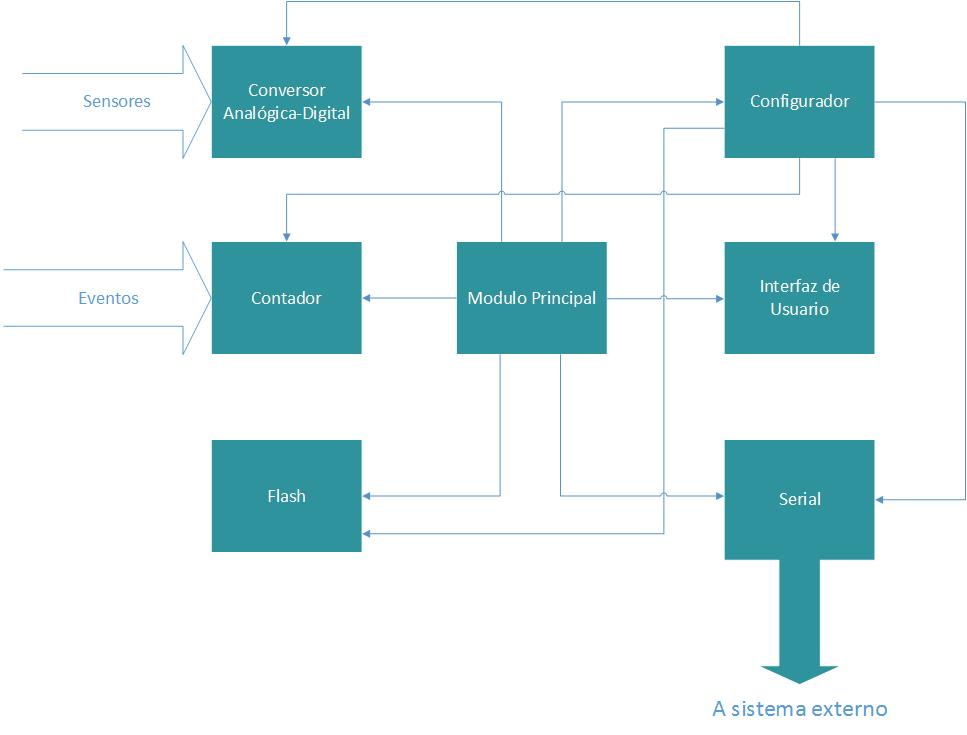
\includegraphics[width=0.80\textwidth, height = 9cm]{Bloques1}
  \caption{\small Diagrama de Bloques 1}\label{fig:bloques1}
\end{figure}

\paragraph{}
El sistema esta compuesto por 7 bloques o módulos separados, manejados por un modulo principal. En la figura \ref{fig:bloques1} se pueden observar estos bloques y la interacción que tienen entre si.
\paragraph{}


\begin{itemize}
  \item El \textbf{Bloque Principal} se encarga ejecutar las funciones del resto de los módulos para dar arranque y ejecución al sistema.
  \item El \textbf{Bloque Conversor Analógico-Digital} principalmente obtiene los datos de los sensores, los procesa, y los envía al modulo principal. Además de esto, configura el funcionamiento del ADC según los parámetros dados por el usuario. El usuario puede elegir la cantidad de pines que va a utilizar como entrada según la cantidad de sensores que quiera medir, puede elegir un nivel de ganancia de amplificación de la señal antes de la conversion, y puede también elegir el modo de obtención de los datos (diferencial o single-ended).
  \item El \textbf{Bloque Contador} se encarga de obtener los valores en los contadores de eventos.
  \item El \textbf{Bloque de Interfaz de Usuario} en este modulo se levanta la interfaz con la que interactua el usuario para establecer los parámetros configurables del sistema.
  \item El \textbf{Bloque Configurador} interactua directamente con el hardware del microcontrolador. Realiza todas las configuraciones necesarias para poder hacer funcionar cada modulo. Es por esto que en el diagrama de bloques se puede ver que este modulo interactua directamente con todos los demás. Inicializa todos los registros pertinentes, el clock del sistema y establece los puertos de entrada y salida.
  \item El \textbf{Bloque Serial} envía los datos por interfaz serial. Puede ser UART o $I^{2}$C.
  \item El \textbf{Bloque Flash} Maneja la unidad de memoria no volátil del sistema. Se utiliza para guardar y cargar configuraciones hechas por el usuario, de forma que puedan cargarse automáticamente al inicio del sistema sin necesidad de volver a configurarlo cada vez que se inicia.
\end{itemize}

% subsubsection diagrama_de_bloques (end)

\subsubsection{Diagramas de caso de uso} % (fold)
\label{ssub:diagramas_de_caso_de_uso}

En la figura \ref{fig:casouso1} se muestra un diagrama de caso de uso del sistema. Los casos de uso son bastante intuitivos, el usuario debe poder configurar todos los aspectos claves del sistema. Este diagrama muestra a grandes rasgos las acciones posibles que pueden hacerse sobre el sistema desde el punto de vista del usuario.

\begin{figure}[h]
  \centering
  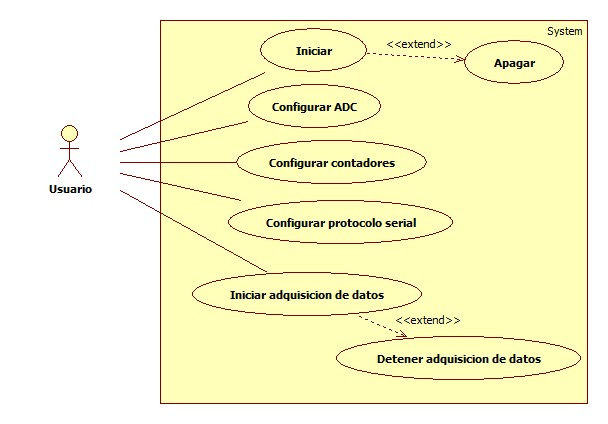
\includegraphics[width=0.80\textwidth, height = 9cm]{CasoUso1}
  \caption{\small Caso de uso 1}\label{fig:casouso1}
\end{figure}

% subsubsection diagramas_de_caso_de_uso (end)

\subsubsection{Diagramas de secuencia} % (fold)
\label{ssub:diagramas_de_secuencia}

Los diagramas de secuencia modelan distintas interacciones entre los componentes de un sistema. En este caso, los dos componentes mas importantes del sistema son el usuario, y el programa principal que recibe las peticiones del usuario a través de la interfaz gráfica, y procesa los pedidos llamando a funciones de otros bloques del sistema. En el primer diagrama (figura \ref{fig:secuencia1}) se modelo una configuración de un pin especifico para medir una entrada analógica. El programa principal, en este caso, debe llamar a funciones del bloque conversor para configurar el pedido del usuario. Luego, el usuario habilita el comienzo de conversion para que el sistema envíe los datos ya digitales por interfaz serial.

\begin{figure}[h]
  \centering
  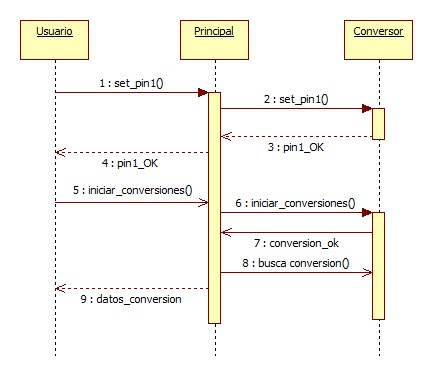
\includegraphics[width=0.50\textwidth, height = 7cm]{Secuencia1}
  \caption{\small Diagrama de secuencia 1}\label{fig:secuencia1}
\end{figure}

El diagrama en la figura \ref{fig:secuencia2} muestra una configuración de un contador. En este sistema, los contadores se inician junto con el arranque mismo del sistema y desde ahí mismo comienzan a contar los eventos que ocurran en el pin que tienen asignado. Es por esto que lo único que hay que hacer es consultar el valor en los registros asociados al contador para obtener la cuenta actual.

El diagrama \ref{fig:secuencia3} muestra una obtención y un guardado de datos de configuración en la memoria flash del microcontrolador. Los datos de configuración son únicamente los pertenecientes al conversor analógico-digital.

\begin{figure}[h]
  \centering
  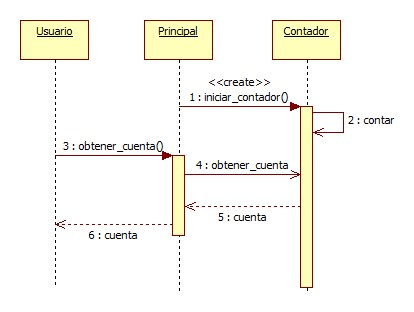
\includegraphics[width=0.50\textwidth, height = 7cm]{Secuencia2}
  \caption{\small Diagrama de secuencia 2}\label{fig:secuencia2}
\end{figure}


\begin{figure}[H]
  \centering
  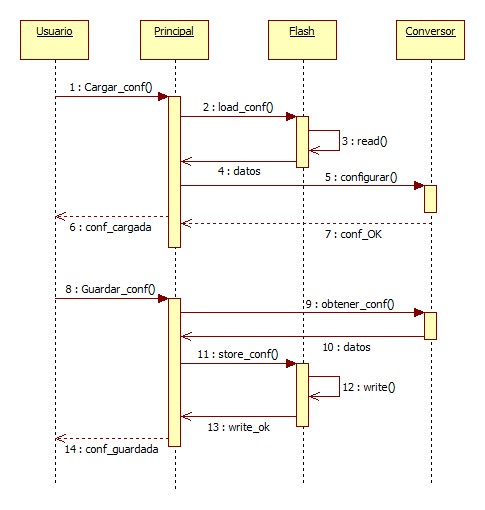
\includegraphics[width=0.60\textwidth, height = 8cm]{Secuencia3}
  \caption{\small Diagrama de secuencia 3}\label{fig:secuencia3}
\end{figure}

% subsubsection diagramas_de_secuencia (end)

% subsection descripción_gráfica_del_sistema (end)

% section diseño_de_software (end)


%Diseño de Hardware
\section{Diseño de hardware} % (fold)
\label{sec:diseno_de_hardware}




Con el microcontrolador seleccionado, se procedió a la etapa de diseño de hardware. La placa de desarrollo C8051F350 (ver sección \ref{sec:silicon_labs_c8051f352}) con la que se contó en el laboratorio donde se trabajo, sirvió de modelo para diseñar el circuito esquemático en la placa a desarrollar.

\subsection{Diagrama de Bloques de Hardware} % (fold)
\label{sub:diagrama_de_bloques_de_hardware}

La primera etapa de diseño consiste en diseñar un diagrama de bloques que ilustre a grandes rasgos la organización del circuito. Luego de esto se realiza el diseño esquemático que consiste en llevar cada bloque a nivel de componente electrónico y realizar la interconexión necesaria entre todos los componentes existentes para lograr el funcionamiento buscado. Los diagramas de bloque y esquemáticos se pueden ver en las figuras \ref{fig:bloquesHW} y \ref{fig:esquematico} Con ayuda del software KiCad (\ref{sub:kicad}), se realizo el diagrama esquemático y la implementación en circuito impreso del esquemático construido.

\begin{figure}[h]
  \centering
  \includegraphics[width=0.80\textwidth, height = 9cm]{bloquesHW}
  \caption{\small Diagrama de bloques del circuito a realizar}\label{fig:bloquesHW}
\end{figure}

Los bloques en la figura \ref{fig:bloquesHW} representan de forma general los distintos modulos a implementar. Las entradas analogicas entran al sistema a traves de filtros que reducen el ruido. Luego ingresan al microcontrolador para ser procesadas. El bloque de GPIO y contadores de eventos es simplemente un grupo de pines direccionados a distintas entradas del microcontrolador. GPIO significa `General Purpose Input Output'. Son 4 pines que se separaron para uso general, por necesidad eventual de necesitarlos. Parte de estos GPIO son los pines contadores de eventos, por lo cual se incluyeron dentro del mismo bloque.

Es posible alimentar el sistema por mediante el programador, o mediante una tension de 3,3V que se obtiene como salida de un regulador de tension, cuya entrada es de 5V. La llave selectora decide si se alimenta el sistema usando la alimentacion por fuente continua de 5V, o por el programador.

% subsection diagrama_de_bloques_de_hardware (end)



\subsection{Diagrama Esquemático} % (fold)
\label{sub:diagrama_esquematico}

La figura \ref{fig:esquematico} muestra el diagrama esquemático del circuito a implementar. El microcontrolador(\ref{sec:silicon_labs_c8051f352}) con el que se trabaja tiene ciertos niveles de tension de operación con el que se trabaja. En principio, se alimenta con una fuente de 5V y 500mA que trabaja en paralelo con un regulador de tension(\ref{sub:regulador_de_tension_lm2937}) que lleve la alimentación a un nivel de 3,3V. Estos 3,3V se utilizan para alimentar al microcontrolador; la tension analógica positiva del conversor; a un integrado MAX232(\ref{sub:driver_max232}) que se utiliza para lograr una interfaz serial entre la UART(\ref{ssub:interfaz_serial}) de la placa y un puerto serial de una PC; y a un led testigo de alimentación.

\begin{figure}[h]
  \centering
  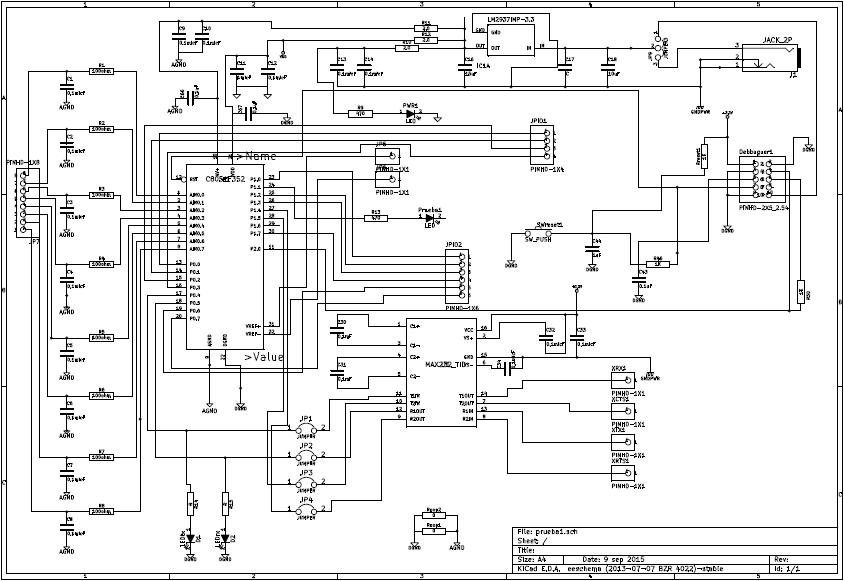
\includegraphics[width=0.95\textwidth, height = 10cm]{esquematico}
  \caption{\small Diagrama esquematico del circuito a realizar}\label{fig:esquematico}
\end{figure}


% subsection diagrama_esquemático (end)

\subsection{Implementación en Circuito Impreso} % (fold)
\label{sub:implementacion_en_circuito_impreso}

Una implementación en circuito impreso consiste simplemente en pasar de un diagrama esquemático al despliegue físico de los componentes reales en una PCB (en inglés, Printed Circuit Board). Para esto, se utilizaron funcionalidades del software KiCad, que también se utilizo para realizar el esquemático del circuito. Una imagen del resultado del despliegue de componentes esta en la figura \ref{fig:PCB1}.

\begin{figure}[h]
  \centering
  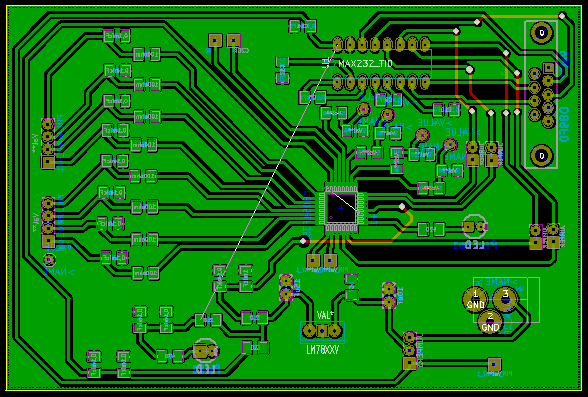
\includegraphics[width=0.95\textwidth, height = 10cm]{PCB1}
  \caption{\small Diagrama del despliegue de componentes}\label{fig:PCB1}
\end{figure}

% subsection implementación_en_circuito_impreso (end)

\subsection{Circuito anexo de programacion} % (fold)
\label{sub:circuito_anexo_de_programacion}

Para programar el microcontrolador, se utiliza un programador de la marca de Silicon Labs hecho para la placa de desarrollo utilizada. Es posible usar este mismo programador en la plataforma a construir, pero es necesario armar un circuito que funcione como interfaz entre la placa del microcontrolador y el programador de la misma. El circuito se muestra en la figura

\begin{figure}[h]
  \centering
  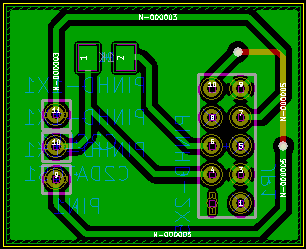
\includegraphics[width=0.20\textwidth, height = 3cm]{PCB2}
  \caption{\small Diagrama del despliegue de componentes del circuito que hace de interfaz entre el programador y la plataforma}\label{fig:PCB2}
\end{figure}

% subsection circuito_anexo_de_programacion (end)

\subsection{Impresión del circuito en placa de cobre} % (fold)
\label{sub:impresion_del_circuito_en_placa_de_cobre}

La impresión de la placa física aun no se implemento. Todavía quedan aspectos que resolver tanto en el diseño del esquemático como el despliegue, y antes de no resolverlos no es posible tener un primer prototipo. Es uno de los objetivos a lograr en las próximas 100 horas de trabajo.

% subsection impresion_del_circuito_en_placa_de_cobre (end)

% section diseno_de_hardware (end)


%Estructura de Software

\section{Estructura del software} % (fold)
\label{sec:estructura_del_software}

El programa esta dividido en 6 módulos que en la mayoría de los casos corresponde a cada bloque en el que esta dividido el sistema, como se muestra en la figura \ref{fig:bloques1}

\subsection{Partes que conforman el software} % (fold)
\label{sub:partes_que_conforman_el_software}

En este momento, el programa entero esta compuesto por 6 módulos. Un modulo principal y otros 5 que definen funciones según los bloques que describen el comportamiento del sistema. El modulo principal ejecuta las funciones de los módulos secundarios.

\paragraph{}
\textbf{Módulos:}
\begin{itemize}
  \item Principal
  \item Conversor
  \item Contador
  \item Interrupciones
  \item Configurador
  \item Interfaz de Usuario
\end{itemize}

% subsection partes_que_conforman_el_software (end)

\subsubsection{Configurador} % (fold)
\label{ssub:configurador}

El configurador se encarga de inicializar todos los parametros necesarios que permiten la operatividad del resto de los módulos. Establece los valores correspondientes para todos los registros pertinentes y configura los puertos seleccionados en el modulo del conversor (Sección \ref{ssub:conversor}) cuando se especifique por parte del usuario.
\subsubsection{Principal}
El modulo principal es la función main, inicializa todo el sistema usando funciones del configurador (Sección \ref{ssub:configurador}) y hace el loop infinito que corre el sistema indefinidamente, obteniendo los comandos del usuario via la interfaz (Sección \ref{ssub:interfaz_de_usuario}).

% subsubsection configurador (end)

\subsubsection{Conversor} % (fold)
\label{ssub:conversor}

El modulo de conversion se encarga de la etapa de obtención y procesado de las señales convertidas del ADC (Sección \ref{sec:adc}).

Las funciones de este modulo se encargan de que la obtención de los datos se corresponda con la configuración dada por el usuario. Es por esto que tiene funciones que se activan en la etapa de configuración del sistema que preparan al mismo para una obtención de datos conforme a los ajustes hechos por el usuario. Estos ajustes se realizan mediante las instrucciones MML mencionadas en la sección \ref{ssub:interfaz_de_usuario} y explicadas con detalle en el apéndice \ref{sec:instrucciones_mml}.

% subsubsection conversor (end)

\subsubsection{Interfaz de Usuario} % (fold)
\label{ssub:interfaz_de_usuario}

En un principio, se comenzó con una interfaz de usuario pensada en forma de un menu principal. La idea era que un pueda acceder a todas las opciones de configuración del sistema desde este menu, ingresando opciones por teclado y cambiando así los parametros. La ventaja de este método es que los errores por parte del usuario se reducen significativamente, dado que no tiene otra opción que elegir entre las opciones que muestra el menu. La desventaja es la complejidad que implica hacer un sistema altamente configurable con una interfaz de este tipo. Esta desventaja fue finalmente la que hizo que se cambiara la interfaz por completo, ya que luego de algunas semanas, las opciones de configuración comenzaron a crecer y se hizo evidente que una interfaz de menu hacia la configuración muy arduosa para el usuario y muy complicada de cambiar y hacer para el programador.Por lo que se cambio a un método con mas libertades para el usuario y menos complejidad para el programador.

La interfaz de usuario actual esta hecha con un lenguaje de especificación denominado "Man Machine Languaje". MML es un lenguaje de especificación que se usa típicamente para estandarizar la interfaz de un sistema para el manejo del mismo desde una consola. Siguiendo el paradigma de MML, lo que se hace es definir una serie de comandos que pueden aceptar una serie de argumentos. Con cada comando y sus argumentos se conforma una orden que ejecuta el procesador. De esta manera, se pueden lograr instrucciones simples que cambian distintos aspectos de la configuración del sistema conforme a las intenciones del usuario. Una descripción completa de las instrucciones hechas hasta el momento se encuentra en el apéndice \ref{sec:instrucciones_mml}. Con esto, es posible configurar todos los aspectos del sistema, sabiendo como operan todas las instrucciones y sus argumentos.

Este esquema de interfaz de usuario esta todavía en proceso. Hasta ahora, las instrucciones descritas en el apéndice \ref{sec:instrucciones_mml} no cubre por completo todas las configuraciones que deberían poder hacerse teniendo en cuenta los requerimientos principales del sistema.

% subsubsection interfaz_de_usuario (end)

\subsubsection{Contador} % (fold)
\label{ssub:contador}

El modulo de contador contiene funciones que devuelven los valores de las cuentas actuales de los contadores en funcionamiento. Por una cuestión de simpleza, los contadores siempre están activos, ya sea que se usen o no. Actualmente se cuenta con tres contadores de eventos. El microcontrolador tiene cuatro timers (Sección \ref{ssub:contador} pero obligadamente uno de ellos debe ser utilizado por el modulo de la interfaz serial UART (Sección \ref{ssub:interfaz_serial}).

Cada contador utilizable tiene una función que simplemente se encarga de obtener el valor de la cuenta en su respectivo timer asociado. Las instrucciones definidas en MML(Sección \ref{ssub:interfaz_de_usuario}) descritas en el apéndice \ref{sec:instrucciones_mml} incluyen las instrucciones GT0, GT1, y GT2, que se utilizan para la obtención del valor de la cuenta actual.


% subsubsection contador (end)

\subsubsection{Interrupciones} % (fold)
\label{ssub:interrupciones}

Este archivo define las rutinas de interrupción para aquellas funcionalidades que se requiere que realicen interrupciones sobre el microcontrolador para condicionar el comportamiento del programa. Actualmente el conversor analógico-digital\ref{ssub:conversor} es el único modulo que realiza interrupciones.


% subsubsection interrupciones (end)
% section estructura_del_software (end)


%Avances con respecto al diseño de hw y sw
\section{Avances con respecto al diseño de software} % (fold)
\label{sec:avances_con_respecto_al_diseno_de_software}

En las primeras 100 horas no fue posible cubrir los requerimientos principales. Los avances obtenidos hasta hoy son los siguientes

\begin{itemize}
  \item Es posible configurar las entradas del ADC en modo single-ended y bipolar
  \item Es posible dar una ganancia de 2 a 128 para cada entrada del conversor
  \item Es posible contar eventos con dos contadores distintos
  \item Es posible modificar la tasa de envío de datos por UART para cada señal convertida por separado
\end{itemize}

% section avances_con_respecto_al_dise~no_de_software (end)

\section{Avances con respecto al diseño de hardware} % (fold)
\label{sec:avances_con_respecto_al_diseno_de_hardware}

\textbf{\underline{ESCRIBITE ALGO ACA}}

% section avances_con_respecto_al_diseno_de_software (end)

%Proyecciones con respecto al futuro
\section{Proyección a futuro} % (fold)
\label{sec:proyeccion_a_futuro}

En las próximas 100 horas de trabajo, el objetivo es finalizar la idea de los diseños propuestos hasta el momento, corregirlos si es necesario, y luego implementar hasta donde se llegue. Si es posible, llegar a tener pruebas de laboratorio funcionando. Probar el dispositivo contentándolo con uno o varios sensores que provean datos crudos, y brindarle la información ordenada a través del protocolo UART \ref{ssub:interfaz_serial} a algún servidor activo que la almacene en una base de datos.

En concreto, los objetivos son los siguientes:
\begin{itemize}
	\item Completar el diseño de hardware
	\item Impresion del circuito en placa de cobre
	\item Ampliar la lista de comandos de la interfaz MML para admitir mayor programabilidad a la plataforma
	\item Añadir mas contadores de eventos utilizando las funcionalidades de Timer y de PCA del microcontrolador utilizado
	\item Añadir la funcionalidad de especificar una frecuencia deseada de muestreo en la adquisición de datos del conversor analógico-digital
	\item Realizar un prototipo del hardware y probarlo con el software desarrollado
	\item Conformar una base de testing que permite probar que todas las funcionalidades de hardware y software funcionen como se espera
\end{itemize}


% section proyección_a_futuro (end)

%conclusiones
\section{Conclusiones de la primera etapa} % (fold)
\label{sec:conslusiones_de_la_primera_etapa}

En esta primera etapa se avanzo principalmente en concepto de investigación y primeros pasos de un proyecto nuevo. Fue en su gran parte una etapa de aprendizaje. Comenzar un proyecto desde cero conlleva una primera etapa lenta con mucha investigación y muchos procesos nuevos en los que hubo falta de destreza al principio, hasta que se adquiere una continuidad que acelera el desarrollo del proyecto. Hasta el momento, es importante destacar que el desarrollo de un proyecto como este en el ambiente de un laboratorio marca una gran diferencia a hacerlo en un ambiente no académico, tanto por el ambiente de trabajo, como la ayuda de profesores, y la ayuda de los mismos compañeros de trabajo dentro del laboratorio. Los avances en las primeras 100 horas de trabajo no son significantes, pero eso se debe mas que nada a una etapa de investigación y primeros pasos extensa. Desde este momento, como se menciona en la sección \ref{sec:proyeccion_a_futuro}, se planea seguir con la implementación del hardware, que según nuestra opinion sera la parte que nos tomara mas trabajo de implementar y verificar que funcione, ya que no somos expertos en hardware y existen muchos conceptos en los que todavía es necesario familiarizarse antes de adentrarse. Por todo lo demás, el interés por el proyecto es alto, y la intención actual es lograr un prototipo que funcione antes de terminar las 200 horas.

% section conclusiones_de_la_primera_etapa (end)
\clearpage

%Apéndice
%\appendix
%\begin{appendices}
%   \addappheadtotoc
%   \appendixpage

\section{Apendices} % (fold)
\label{sec:apendices}


\appendix
\section{Instrucciones MML} % (fold)
\label{sec:instrucciones_mml}


\subsection{SSE (Set Single Ended)} % (fold)
\label{sub:sse_set_single_ended}


\textbf{Formato:} SSE,[1]

\textbf{Descripción:}
Establece el pin ingresado en modo single ended.

\textbf{Limitaciones:}
\begin{itemize}
  \item Un solo argumento
  \item El argumento es un byte par comprendido entre 0 y 7
\end{itemize}

\textbf{Ejemplo:}

SSE,4: Establece el pin 4 del ADC en modo single ended
% subsection sse_set_single_ended (end)


\subsection{SDI (Set Diferencial)} % (fold)
\label{sub:sdi_set_diferencial}


\textbf{Formato:} SDI,[1]

\textbf{Descripción:}
Establece el pin ingresado y el pin siguiente a ese en numero en modo diferencial

\textbf{limitaciones:}
\begin{itemize}
  \item un solo argumento
  \item el argumento es un byte par comprendido entre 0 y 6
\end{itemize}

\textbf{ejemplo:}

SDI,2: setea los pines 2 y 3 en modo diferencial

% subsection sdi_set_diferencial (end)
\subsection{SGA (Set Ganancia)} % (fold)
\label{sub:sga_set_ganancia}


\textbf{Formato:} SGA,[1]

\textbf{Descripción:}
Establece la ganancia del ADC según el argumento a la potencia de 2

\textbf{Limitaciones:}
\begin{itemize}
  \item Un solo argumento
  \item El argumento es un byte comprendido entre 0 y 7
\end{itemize}

\textbf{Ejemplo:}

SGA,3: Establece la ganancia en $2^{3} = 8$
% subsection sga_set_ganancia (end)


\subsection{GT0 (Get Timer 0)} % (fold)
\label{sub:gt0_get_timer_0}


\textbf{Formato:} GT0[0]

\textbf{Descripción:}
Obtiene el valor actual de la cuenta de los eventos digitales monitoreados por timer0

\textbf{Limitaciones:}
\begin{itemize}
  \item No lleva argumentos
\end{itemize}

% subsection gt0_get_timer_0_ (end)
\subsection{GT2 (Get Timer 2)} % (fold)
\label{sub:gt2_get_timer_2}

\textbf{Formato:} GT2[0]

\textbf{Descripción:}
Obtiene el valor actual de la cuenta de los eventos digitales monitoreados por timer2

\textbf{Limitaciones:}
\begin{itemize}
  \item No lleva argumentos
\end{itemize}

% subsection gt2_get_timer_2_ (end)
\subsection{ST (Start)} % (fold)
\label{sub:st_start}


\textbf{Formato:} ST[0]

\textbf{Descripción:}
Guarda los cambios, sale del modo de configuración y comienza a correr el programa

\textbf{Limitaciones:}
\begin{itemize}
  \item No lleva argumentos
\end{itemize}

% subsection st_start_ (end)


% section instrucciones_mml (end)

\section{Componentes Electrónicos Utilizados} % (fold)
\label{sec:componentes_electronicos_utilizados}


% \subsection{Optoacoplador T2103} % (fold)
% \label{ssub:optoacoplador_t2103}



% subsubsection optoacoplador_t2103 (end)


\subsection{Regulador de Tension LM2937} % (fold)
\label{sub:regulador_de_tension_lm2937}

Es un regulador de tension positivo capaz de soportar una corriente de carga de 500mA. Desarrollado por Texas Instruments. Ideal para aplicaciones de automatización. Tiene protección intrínseca contra corrientes inversas, y protección contra cortocircuitos. \\

\textbf{Mas información:} http://www.ti.com/lit/ds/symlink/lm2937.pdf

% subsection regulador_de_tension_lm2937 (end)

\subsection{Driver MAX232} % (fold)
\label{sub:driver_max232}

Es un driver receptor/emisor que incluye un voltaje capacitivo generador para proveer voltajes a niveles TTL de una alimentación de 5V. Un receptor convierte entradas de tipo s TIA/EIA-232-F a niveles TTL/CMOS. Tiene una histeresis típica de 0.5V. \\


\textbf{Mas información:} http://www.ti.com/lit/ds/symlink/max232.pdf

% subsection driver_max232 (end)





% section componentes_electrónicos_utilizados (end)

\section{Software Utilizado} % (fold)
\label{sec:sofware_utilizado}


\subsubsection{$\mu$Vision 4} % (fold)
\label{ssub:uvision_4}

$\mu$Vision 4 es un entorno de desarrollo de programación desarrollado por KeilARM. Esta pensado para construcción de programas en C destinados a correr sobre sistemas embebidos, como es el caso de una Silicon Labs C8051F350. Confecciona todos los archivos fuente de un proyecto y los arma en un único ejecutable, que luego puede cargarse al microcontrolador para su ejecución. También permite la opción de debugging. \\

\textbf{Mas información:}$\mu$Vision IDE Overview ( http://www.keil.com/uvision/default.asp )


% subsubsection uvision_4 (end)

\subsection{KiCad} % (fold)
\label{sub:kicad}

Kicad es una herramienta de software abierto que permite crear circuitos electrónicos desde la etapa de diseño hasta la implementación en circuito impreso. Permite la generación de los archivos necesarios para generar la placa PCB impresa utilizando una fresadora o ruteadora.  \\


\textbf{Mas información:} KiCad EDA: A Cross Platform and Open Source Electronics Design Automation Suite ( http://kicad-pcb.org/help/documentation )


% subsection kicad (end)



% section software_utilizado (end)

\clearpage

% section apendices (end)


%Bibliografía
% Bibliografía.
%-----------------------------------------------------------------
\begin{thebibliography}{99}

\bibitem{bib:datasheet} Silicon Laboratories \emph{C8051F351/2/3} 8K ISP Flash MCU Family (http://www.keil.com/dd/docs/datashts/silabs/c8051f35x.pdf)

\end{thebibliography}






%\begin{equation}\label{eq:area}
%  S = \pi r^2
%\end{equation}
%Uno puede referirse a ecuaciones así: ver ecuación (\ref{eq:area}).
%También se pueden mencionar secciones de la misma forma: ver sección
%\ref{sec:nada}. O citar algo de la bibliografía: \cite{Cd94}.




\end{document} 